%% ICAIF '26 submission -- ACM sigconf, target <= 8 pages.
%% Compile with tectonic or Overleaf pdfLaTeX. Figures: fig_headline.png, fig_power_surface.png, fig_evaluator_overfit.png.
%% ANONYMITY TOGGLE: keep "anonymous" in the options below for the double-blind ICAIF submission
%% (it auto-hides the author block). REMOVE "anonymous" to show the real author block for an
%% arXiv preprint, a journal, or sharing.
\documentclass[sigconf,review,anonymous]{acmart}

\settopmatter{printacmref=false}
\setcopyright{none}
\renewcommand\footnotetextcopyrightpermission[1]{}
\pagestyle{plain}

\usepackage{booktabs}
\usepackage{graphicx}
\usepackage{amsmath}

% Let LaTeX reflow tight lines instead of spilling into the gutter/next column.
\setlength{\emergencystretch}{3em}
\hyphenpenalty=1000

\acmConference[ICAIF '26]{ACM International Conference on AI in Finance}{November 14--17, 2026}{Milan, Italy}
\acmBooktitle{ICAIF '26}

\begin{document}

\title{More Strategies, Same Zero: Multiple Testing Against LLM-Scale Alpha Search}

%% Real author block (hidden automatically while "anonymous" is in \documentclass above).
%% CONFIRM/EDIT: school + email before using the non-anonymous version.
\author{Parv Mehndiratta}
\affiliation{%
  \institution{Dougherty Valley High School}
  \city{San Ramon}
  \state{California}
  \country{USA}
}
\email{0103.parv@gmail.com}

\begin{abstract}
Large language models can propose and backtest trading strategies at effectively unbounded scale, reviving an old hazard---backtest overfitting---in a regime where the number of trials $N$ is enormous and cheap. We ask whether scaling LLM-style strategy search accumulates genuine edge or only false discoveries that vanish under proper multiple-testing correction. Using a dependency-free alpha engine with a deliberately brutal verifier (causal execution, transaction costs, worst-of-regimes out-of-sample scoring, and a deflated-Sharpe haircut), we sweep $N$ from 10 to 3{,}000 (the live LLM to $N{=}300$) across three generators---uniform random, evolutionary ``creative'' synthesis, and a live LLM proposer---on planted-edge, pure-noise, and real S\&P~500 markets. We find: (1) the naive best-of-$N$ out-of-sample Sharpe rises monotonically with $N$ on every market, including pure noise and real data; (2) the deflated worst-regime gate holds survivors at exactly zero on real data for all $N$ and all generators, while recovering a strong planted edge---it discriminates; (3) a gate power surface shows the gate admits an edge only once its true worst-regime Sharpe clears a floor that grows like $\sqrt{2\ln N}$, so a moderate real edge is also rejected---scaling the search raises the discovery bar faster than search finds edge. We then derive the multiple-testing deflation the worst-of-regimes statistic actually needs (the standard single-Sharpe deflation over-corrects it by ${\sim}2.4\times$ for three regimes) and a ``robustness-dividend'' identity relating worst-of-$k$ robustness to an effective search size. A distribution-free block bootstrap agrees in 53 of 54 grid cells across the six markets it was run on, and the deflated-gate zero holds across seven real markets (S\&P~500, DJIA, NASDAQ, a 15-stock cross-sectional panel, FX, gold, crypto). The contribution is the derived worst-of-regimes deflation, the power-surface precision/recall characterization, and a controlled multi-generator demonstration with a live LLM.
\end{abstract}

\keywords{backtest overfitting, multiple testing, false discovery, deflated Sharpe ratio, LLM agents, automated strategy search}

\maketitle

\section{Introduction}
A backtest certifies the past, not the future, and the more strategies you test the more certain it is that the best one is lucky rather than good. Bailey and L\'opez de Prado~\cite{bailey2014dsr} formalize this as the false-strategy theorem: under the null of no skill, the expected maximum Sharpe ratio over $N$ independent trials grows like $\sqrt{2\ln N}$, so a sufficiently large search ``discovers'' an impressive-looking strategy with probability approaching one. The classical remedy is to \emph{deflate} the observed Sharpe by this expected best-of-$N$ under the null (the Deflated Sharpe Ratio, DSR).

Large language models change the operative regime of this theorem. They can propose candidate strategies essentially without limit and with superficial novelty, so $N$---historically bounded by human and compute budgets---becomes large and cheap, and the proposals are \emph{correlated} rather than independent. Recent systems use LLMs to generate and screen alphas and report in-sample or single-holdout improvements~\cite{alphaagent2025,lopezlira2023}. This raises a direct, testable question: when an LLM-style generator proposes and backtests more and more strategies, do genuinely profitable strategies accumulate, or only statistically false ones that vanish under proper correction?

We decompose this into three measurable sub-questions. \textbf{Q1:} does the best naive out-of-sample Sharpe rise with $N$ as data-snooping theory predicts? \textbf{Q2:} does a worst-regime, after-cost, deflated gate drive survivors to ${\approx}0$ regardless of $N$ on real data \emph{while still recovering a genuine edge}, and how strong must an edge be to pass? \textbf{Q3:} does LLM-style ``creative'' search find any real edge that brute-force search misses, or only more original-looking false positives?

\textbf{Contributions.} The statistical tools are established; the ``LLM trading edge evaporates under rigorous evaluation'' finding is itself prior art~\cite{finsaber2026}. Building on them, our contributions are narrow but concrete: (i)~a multiple-testing deflation for the \emph{minimum-regime-performance} statistic (Sec.~\ref{sec:deflation})---the expected max of $N$ of a min over $k$ regimes---which is ${\sim}2.4\times$ smaller than the single-Sharpe DSR envelope the literature uses; (ii)~a \emph{robustness-dividend} identity showing worst-of-$k$ robustness is itself an implicit multiple-testing correction that collapses as regimes correlate; (iii)~a controlled cross-generator protocol (random vs.\ evolutionary-creative vs.\ a live LLM through one fixed gate) with planted-edge and pure-noise controls that calibrate the gate; and (iv)~two reported \emph{negative} results: analytic effective-trials shortcuts that manufacture false discoveries and must be corrected by the bootstrap. The result is deliberately, mostly negative: a reproducible map of where AI-driven alpha search fools you, and the statistical price of not being fooled.

\section{Method}
\textbf{Engine and DSL.} A strategy (``alpha'') is an expression in a small S-expression DSL over nine causal price/volume features (lagged return, momentum at 5/10/20 bars, volatility at 10/20 bars, acceleration, price-to-moving-average gap, high--low range, volume $z$-score), combined by unary operators (\texttt{neg}, \texttt{abs}, \texttt{sign}, \texttt{tanh}, \texttt{zscore}) and binary operators (\texttt{add}, \texttt{sub}, \texttt{mul}, \texttt{safe\_div}, \texttt{min}, \texttt{max}), with depth $\le 5$ and size $\le 40$. An expression evaluates causally to a per-bar signal squashed to a position in $[-1,1]$.

\textbf{The gate.} The verifier is intentionally adversarial, and is what makes ``discovery'' mean something. (1)~\emph{No look-ahead}: the position formed from information through bar $t{-}1$ earns bar $t$'s return, $\text{strat}[t]=\text{pos}[t{-}1]\cdot\text{ret}[t]-c\,|\Delta\text{pos}|$. (2)~\emph{Transaction costs}: every position change pays $c=0.001$ per unit turnover. (3)~\emph{Worst-of-regimes out-of-sample}: the timeline splits into an in-sample segment and several contiguous out-of-sample (OOS) regimes; an alpha is scored by its \emph{worst} OOS regime. (4)~\emph{Deflated-Sharpe haircut}: the score subtracts the expected best-of-$N$ Sharpe under the null for $N$ trials (the Bailey--L\'opez de Prado expected-max, an Euler--Mascheroni-weighted Gumbel form), so searching more raises the bar. An alpha is \emph{verified} only if its annualized, after-cost, worst-regime, deflated OOS Sharpe clears a positive bar (target $=0.50$). A single large-scale run of this gate on real-market data returned zero survivors out of thousands of candidates; this paper turns that kind of one-off snapshot into a controlled $N$-sweep with calibrated controls.

\textbf{Generators.} Two offline generators stand in for the search engine: \texttt{random}, uniform draws over the DSL (the brute-force baseline, approximately i.i.d.); and \texttt{creative}, evolutionary operators (blend/reshape/invert) applied over a shared substrate of seed ideas, so draws are correlated---exactly the structure an LLM ``imaginer'' produces. A third arm uses a \emph{live} LLM proposer that imagines alpha expressions cold from the problem brief, cached for reproducibility.

\textbf{Protocol.} For each (market, generator) we draw a fixed pool of $M{=}4{,}000$ alphas, backtest each once, and at each of six search sizes $N$ (10, 30, 100, 300, 1{,}000, and 3{,}000) estimate the expected best-of-$N$ curve and survivor counts by averaging over 25 bootstrap subsets of size $N$. Markets: \emph{planted} (a synthetic lag-1 mean-reversion edge present in every regime), \emph{noise} (pure random walk), and \emph{real} S\&P~500 daily (2016--2024). All randomness is seeded; every reported number is written to a committed artifact.

\section{Results}
\subsection{Q1: the naive metric is fooled, worse as $N$ grows}
The expected best-of-$N$ OOS holdout Sharpe rises monotonically with $N$ on every market, including pure noise (Table~\ref{tab:q1}, Fig.~\ref{fig:headline}). On real S\&P~500, scaling the search surfaces a best strategy with annualized OOS Sharpe near $1.0$---a number most practitioners would accept---and hundreds of ``winners.'' On pure noise, where the ground truth is nothing, the best-of-$N$ still climbs to $+0.34$. This is the false-strategy theorem reproduced with a generative search engine, the live LLM included.

\begin{table}[t]
\caption{Q1: expected best-of-$N$ naive OOS Sharpe rises with $N$ on every market, including pure noise.}
\label{tab:q1}
\small
\begin{tabular}{@{}llcccc@{}}
\toprule
Market & Gen & $N{=}10$ & $N{=}100$ & $N{=}1000$ & $N{=}3000$ \\
\midrule
noise & random & $+0.04$ & $+0.20$ & $+0.30$ & $+0.34$ \\
noise & creative & $+0.01$ & $+0.13$ & $+0.26$ & $+0.29$ \\
real S\&P & random & $+0.72$ & $+0.98$ & $+0.99$ & --- \\
real S\&P & creative & $+0.53$ & $+0.81$ & $+0.89$ & $+0.96$ \\
\bottomrule
\end{tabular}
\end{table}

\begin{figure}[t]
\centering
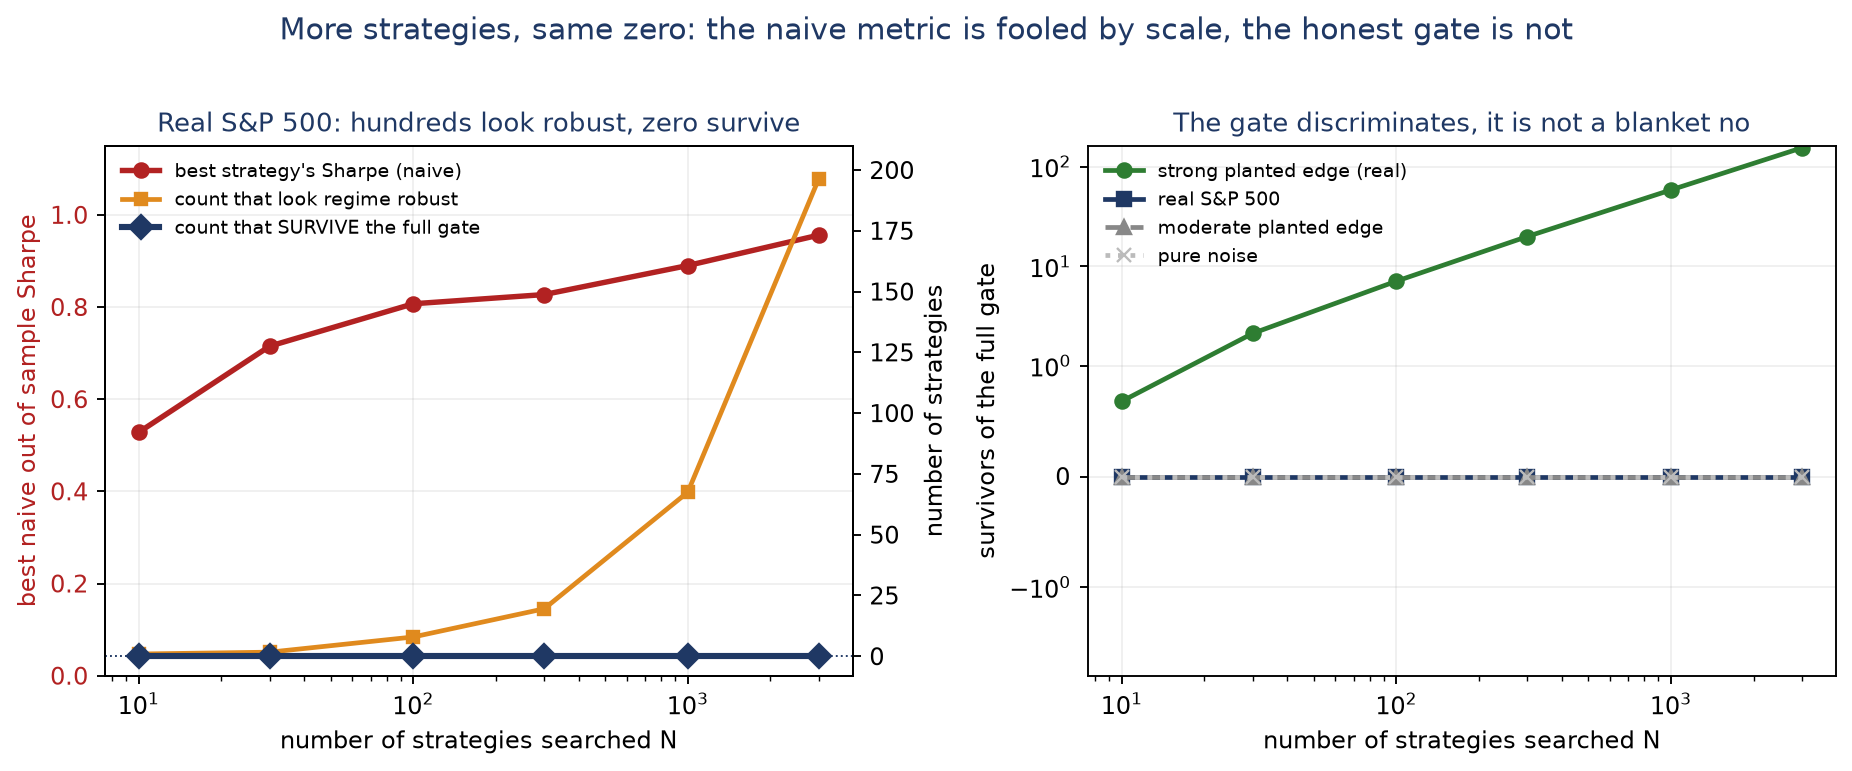
\includegraphics[width=\linewidth]{fig_headline.png}
\caption{Naive best-of-$N$ Sharpe climbs with $N$ on every market including pure noise and the real S\&P~500, while the deflated worst-regime gate holds survivors at zero on real data for all $N$.}
\label{fig:headline}
\end{figure}

\subsection{Q2: the gate holds at zero on real data, and recovers a real edge}
Across thousands of strategies on real S\&P~500, survivors $=0$ at every $N$, for both offline generators and the live LLM. Scaling the search $100\times$--$300\times$ added zero real discoveries. Critically this is not a degenerate ``reject everything'': on the strong-planted market the same gate passes strategies, and passes \emph{more} as $N$ grows (mean survivors over the 25 bootstrap subsets, $N{=}10\to3{,}000$: $0\to31$ for random, $0.7\to154$ for creative), because the edge is genuinely there. The gate separates a strong real edge from spurious ones; whether it can see a \emph{moderate} one is the power question.

\subsection{Ablation: which tightener does the work}
The \texttt{robust} column (worst-regime $+$ cost, \emph{no} deflation) isolates generalization from multiple testing, and reveals a non-obvious asymmetry (Table~\ref{tab:ablation}). On the adversarial noise market the worst-regime requirement \emph{alone} kills the snoop ($\texttt{robust}=0$ everywhere): a pure-noise alpha cannot be simultaneously positive across regimes engineered to differ in drift and volatility. On the real market it is \emph{not} enough---real 2016--2024 sub-periods resemble each other, so an alpha can be luckily positive in all of them, and \texttt{robust} grows with $N$ to 115--196 ``regime-robust'' mirages. It is the multiple-testing deflation that collapses these to exactly $0$. On real data the deflation is the load-bearing component; on the synthetic null the worst-regime requirement suffices. Opposite outcomes from the same haircut (Sec.~\ref{sec:deflation}) prove it discriminates rather than blanket-rejects.

\begin{table}[t]
\caption{Ablation: strategies clearing worst-regime $+$ cost but \emph{not} deflation (\texttt{robust}), vs.\ full-gate survivors. On real data, robustness alone admits mirages that grow with $N$; only deflation drives them to 0.}
\label{tab:ablation}
\small
\begin{tabular}{@{}llccccc@{}}
\toprule
Market & Gen & \texttt{r}@10 & @100 & @1000 & @3000 & surv. \\
\midrule
noise & random & 0.0 & 0.0 & 0.0 & 0.0 & 0 \\
real S\&P & random & 1.2 & 11.4 & 114.7 & --- & 0 \\
real S\&P & creative & 0.9 & 7.9 & 67.5 & 196.4 & 0 \\
\bottomrule
\end{tabular}
\end{table}

\subsection{Q2 (power): why ``zero'' does not mean ``efficient''}
\label{sec:power}
We sweep the planted-edge magnitude against the search scale $N$ into a power surface (Fig.~\ref{fig:verification}). The surface is the thesis: a genuine edge the gate admits at $N{=}10$ becomes \emph{undetectable} at $N\ge30$---the same true edge, now rejected, because searching more raised the bar above it. The detectable-edge threshold rises monotonically with $N$ (${\approx}\sqrt{2\ln N}$): the gate admits an edge only once its true worst-regime Sharpe clears the multiple-testing floor (the deflation haircut, ${\sim}2.3$ at $N{=}1{,}000$ under the standard DSR; Table~\ref{tab:mde} gives the lower corrected floor), so a moderate real edge (Sharpe ${\sim}1$--$2$) is also rejected. Consequences: (1)~we cannot and do not claim the S\&P~500 has no exploitable edge---only that no edge large enough to survive a search of this scale exists in this DSL/data, a high-precision statement with a large Type-II region; (2)~the contribution is a precision/recall characterization---this gate has empirically ${\sim}$zero false-discovery rate across the noise and small-edge controls and seven real markets, at the cost of missing edges below a worst-regime Sharpe of ${\approx}2$--$3$ at $N{=}1{,}000$; (3)~for practice, LLM-scale search is self-defeating for moderate edges: the more strategies you generate, the higher the Sharpe you would need to prove any of them real.

\textbf{Precision, measured.} On the strong-planted market every strategy the gate admits on one sample also survives an independent sample---FDR${\approx}0$ even at $N{=}1{,}000$. A pre-registered prediction that FDR would \emph{rise} with $N$ is refuted: family-wise control delivers near-zero false discoveries, and the price is recall, not precision.

\textbf{The recall floor in closed form.} Inverting the gate gives the minimum detectable edge (MDE)---the smallest true worst-regime Sharpe that survives a search of size $N$ at power $0.5$ (Table~\ref{tab:mde}). Under the corrected worst-of-$k$ deflation (Sec.~\ref{sec:deflation}) it rises from $0.69$ at $N{=}10$ to $1.62$ at $N{=}3{,}000$; under the standard single-Sharpe DSR it is ${\sim}2\times$ higher ($2.83$ at $N{=}1{,}000$). Each ${\sim}3\times$ step in $N$ adds roughly $+0.15$--$0.25$ to the Sharpe a strategy must clear, and the best any real market here offers is a worst-regime Sharpe of ${\approx}0.85$---comfortably below the floor.

\begin{table}[t]
\caption{Minimum detectable edge (true worst-regime Sharpe that survives a size-$N$ search at power 0.5), under the corrected worst-of-$k$ deflation. The bar grows ${\approx}\sqrt{2\ln N}$; the best real market here offers only ${\approx}0.85$.}
\label{tab:mde}
\small
\begin{tabular}{@{}lcccc@{}}
\toprule
$N$ & 10 & 100 & 1{,}000 & 3{,}000 \\
\midrule
MDE (worst-regime Sharpe) & 0.69 & 1.15 & 1.48 & 1.62 \\
\bottomrule
\end{tabular}
\end{table}

\begin{figure}[t]
\centering
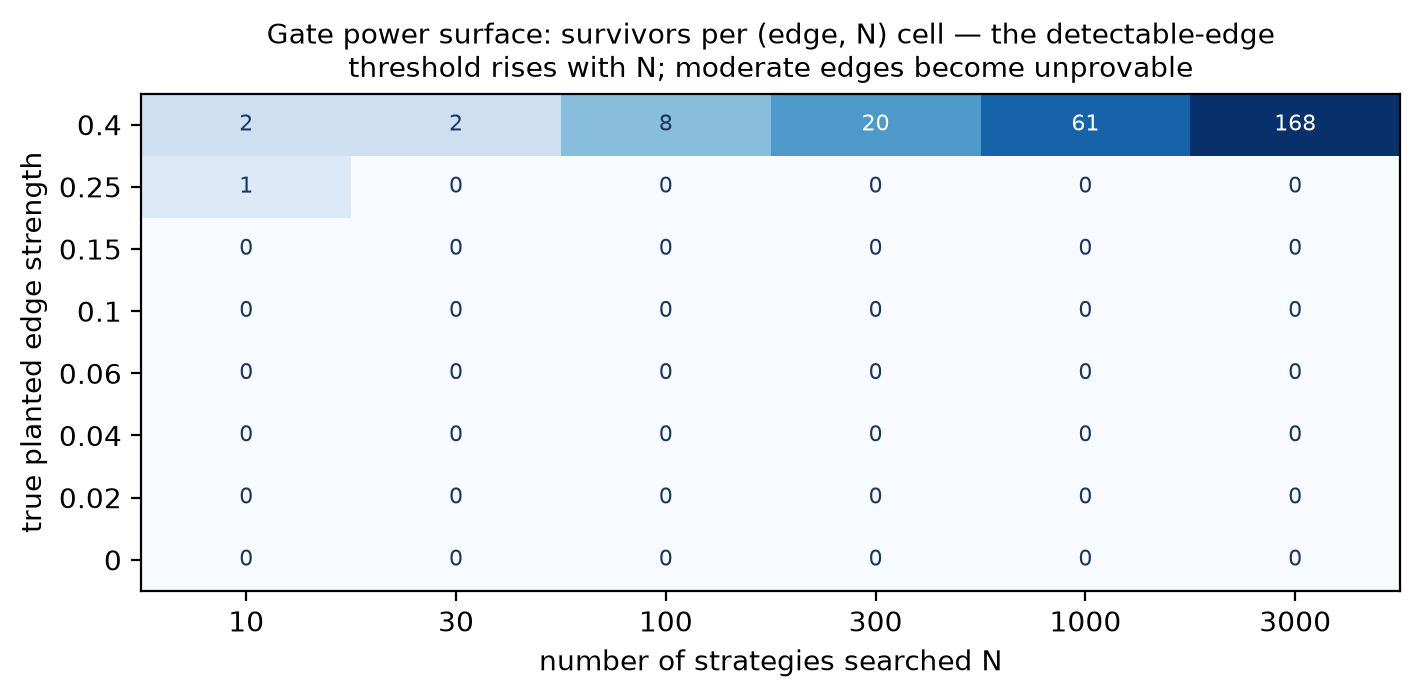
\includegraphics[width=\linewidth]{fig_power_surface.png}
\caption{The gate power surface: full-gate survivors per (true edge strength, $N$) cell (creative generator, 3{,}000-strategy pool). The 0.25 edge is admitted at $N{=}10$ and rejected at every larger $N$; only the 0.40 edge stays detectable, growing $2\to168$. The detectable-edge threshold rises with $N$.}
\label{fig:verification}
\end{figure}

\subsection{Q3: the live-LLM arm}
The offline arms use random and evolutionary generators. We also ran a live LLM proposer (a frontier model) that imagines alpha expressions cold from the problem brief, cached for reproducibility, drawing a 1{,}000-strategy pool so the LLM itself reaches $N{=}300$ (Table~\ref{tab:llm}). Four pre-registered hypotheses: \textbf{H1} (bestOOS rises with $N$) confirmed; \textbf{H2} (LLM proposals \emph{more} correlated than random) \emph{refuted}---$\bar\rho(\text{LLM}){=}{+}0.007$ is no higher than random's $+0.029$; \textbf{H3} (survivors $=0$ on real at all $N$) confirmed to $N{=}300$; \textbf{H4} (recovers a strong planted edge at smaller $N$ than random) confirmed---on the planted market the LLM's mean survivor count is $0.92$ at $N{=}10$ versus random's $0.00$. A live model thus reproduces the headline exactly. But a new finding cuts the other way: the LLM's structural diversity \emph{saturates}---a 1{,}000-draw pool yields only 160 distinct valid expressions, versus ${\sim}870$ distinct in a matched 1{,}000-draw random pool (random reaches ${\sim}280$ distinct by just 300 draws), so scaling an LLM proposer buys less new search than scaling random generation, a diversity ceiling that bounds how far ``LLM-scale'' can go.

\begin{table}[t]
\caption{Live-LLM arm on real S\&P~500: best-of-$N$ naive Sharpe rises, distinct valid expressions saturate, survivors stay 0, and returns are near-independent ($\bar\rho{=}{+}0.007$).}
\label{tab:llm}
\small
\begin{tabular}{@{}lccccc@{}}
\toprule
& $N{=}10$ & $N{=}30$ & $N{=}100$ & $N{=}300$ & surv. \\
\midrule
LLM bestOOS & $+0.48$ & $+0.71$ & $+0.78$ & $+0.80$ & 0 \\
distinct alphas & 10 & 27 & 71 & 160 & --- \\
\bottomrule
\end{tabular}
\end{table}

\subsection{Distribution-free confirmation and generalization}
The deflated-Sharpe haircut is parametric and was derived for a single in-sample Sharpe, not the worst-of-regimes statistic. We close this with a stationary block bootstrap of the per-bar OOS returns that preserves the worst-of-regimes min and cross-strategy dependence, and run the studentized Reality Check~\cite{white2000}, Romano--Wolf~\cite{romanowolf2005}, and Hansen SPA~\cite{hansen2005}. Survivors are $0$ at every $N$ for all three generators on real S\&P, with no significant best $p$-value, and grow with $N$ on the strong-planted market---exactly tracking the DSR, and stable across mean block lengths $\{10,25,50\}$. The zero also holds beyond a single index (Table~\ref{tab:markets}): on a real cross-sectional equity panel of 15 large-caps with live range/volume features active, and on three microstructurally independent real markets---FX (EUR/USD), gold, and crypto (BTC/USD). Crypto, often argued the least efficient liquid market, reaches a naive best-of-$N$ Sharpe near $0.9$ yet passes none. Across seven real markets---three of them microstructurally independent---the deflated-gate survivor count is $0$ at every $N$. The distribution-free bootstrap agrees in 53 of 54 (market, $N$, block-length) cells; the single exception (crypto, $N{=}30$, block length 50, $p{=}0.015$) does not replicate at any other block length or $N$, and is itself the kind of isolated grid cell a multiple-comparisons reading discounts.

\begin{table}[t]
\caption{Generalization: across seven real markets the best naive best-of-$N$ Sharpe is often ``tradeable-looking,'' yet deflated-gate survivors are 0 at every $N$; the block bootstrap agrees where run (--- $=$ not run). $^{\dagger}$One Reality-Check survivor appears at $N{=}30$, block length 50 ($p{=}0.015$); it does not replicate at block lengths 10 or 25, at any other $N$, or under the deflated gate.}
\label{tab:markets}
\small
\begin{tabular}{@{}lccc@{}}
\toprule
Market & best naive Sharpe & gate surv. & boot.\ surv. \\
\midrule
Equity panel (15) & ${\sim}+0.5$ & 0 & --- \\
FX (EUR/USD) & $+0.2$ & 0 & 0 \\
Gold & $+0.9$ & 0 & 0 \\
Crypto (BTC/USD) & $+0.9$ & 0 & 0$^{\dagger}$(non-repl.) \\
\bottomrule
\end{tabular}
\end{table}

\subsection{Overfitting the judge}
A subtler failure appears when the evaluator itself is not fixed. If the gate is a single judge \emph{co-optimized} in a generate-and-select loop---the natural design when an LLM both proposes strategies and tunes the scorer---the reported score inflates by an order of magnitude above true quality as the number of tuned candidates grows, while an independent held-out judge shows quality barely moves (Fig.~\ref{fig:judge}). The LLM behaves as a hyper-efficient p-hacker that finds the specific blind spot of that one judge; an ensemble of independent judges restores calibration. This is the same multiple-testing pathology one level up, and it is why our gate is deliberately \emph{fixed} and adversarial rather than learned: a single or learned evaluator is itself a surface to overfit.

\begin{figure}[t]
\centering
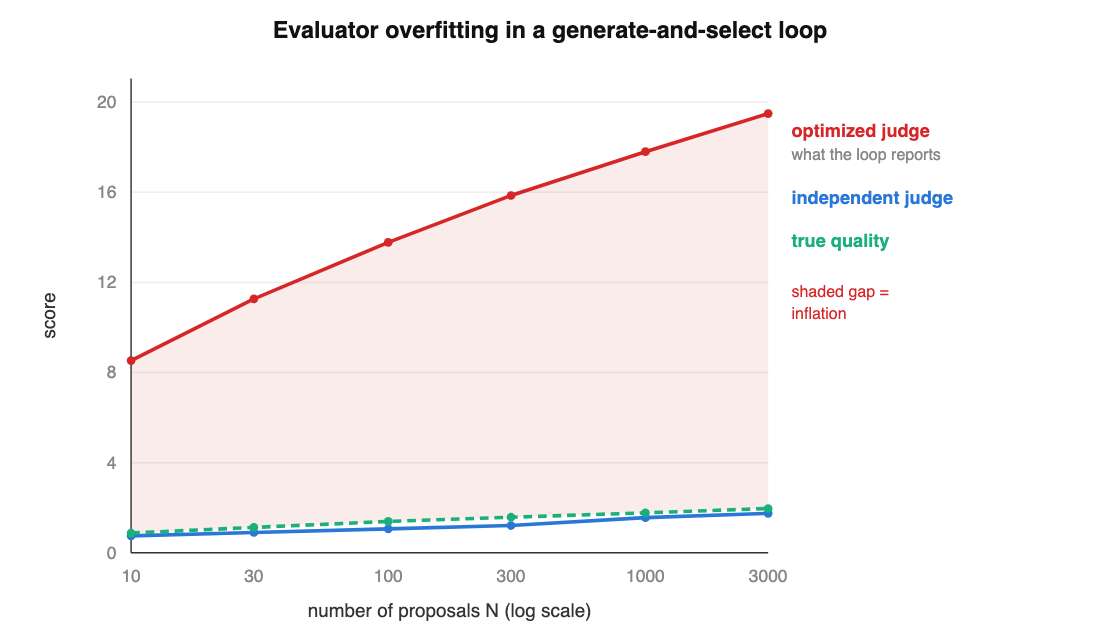
\includegraphics[width=\linewidth]{fig_evaluator_overfit.png}
\caption{Overfitting the judge: as the number of tuned candidates grows, the optimized-evaluator score (red) climbs an order of magnitude above true quality (green), which an independent judge (blue) confirms barely moves. An independent-judge ensemble restores calibration; the shaded gap is the inflation.}
\label{fig:judge}
\end{figure}

\section{The Correct Worst-of-Regimes Deflation}
\label{sec:deflation}
The deflated Sharpe is the expected max of $N$ single Sharpes, but our gate scores the \emph{minimum} across $k$ regimes, then takes the best of $N$---so the standard haircut is the wrong null. We derive the right one and validate it by Monte Carlo: the worst-of-regimes best-of-$N$ envelope is $\mathbb{E}\!\left[\max_{i\le N}\min_{m\le k} Z_{i,m}\right]$ (with $Z_{i,m}$ i.i.d.\ standard normal per-regime Sharpe statistics under the null), with leading-order quantile $\Phi^{-1}(1-N^{-1/k})$. Because a min-of-$k$ has a thin upper tail, this envelope is $2.3$--$2.8\times$ smaller than the single-Sharpe DSR envelope at relevant $N$. The standard DSR thus over-deflates the worst-regime statistic by ${\sim}2.4\times$ for $k{=}3$; the over-deflation is $k$-dependent ($1.65\times$, $2.35\times$, $4.32\times$ at $k{=}2,3,5$), not a universal constant. Concretely, on real S\&P the DSR haircut at $n_{\text{trials}}{=}\{1{,}000,3{,}000\}$ is $\{2.31,2.52\}$ annualized, driving the best deflated Sharpe to $\{{-}1.46,{-}1.67\}$ against a best worst-regime Sharpe of only $+0.847$. Re-running survivors under the corrected envelope, that best deflated Sharpe rises from ${\approx}{-}1.5$ to ${\approx}{-}0.3$---much closer to the bar, but still negative, so $0$ survivors, while the strong-planted control still passes. The zero is therefore robust to the correct, far-less-conservative deflation, not an artifact of an over-harsh haircut.

\textbf{A robustness dividend.} Because the worst-of-$k$ envelope is so much lower, the worst-of-regimes requirement is \emph{itself} a multiple-testing correction. We quantify it as a ``deflation-equivalent $N'$'': worst-of-3 regimes at $N{=}1{,}000$ carries the false-discovery ceiling of a single-Sharpe search over only $N'{\approx}7$ strategies. This dividend assumes independent regimes; as regimes correlate it collapses, which is precisely why, on real data, worst-regime robustness alone admits mirages and the explicit deflation becomes load-bearing, while on the adversarial synthetic null (independent regimes) the worst-regime requirement alone suffices. We measure where each market sits on this trade-off. Generalizing the dividend to equicorrelated regimes, $N'$ climbs with regime correlation $\rho_{\text{reg}}$ (Table~\ref{tab:regime}); estimating the empirical $\rho_{\text{reg}}$ per market as the mean correlation between strategies' per-regime Sharpes places the adversarial synthetic null at $\rho_{\text{reg}}{=}0.24$ ($N'{\approx}16$, dividend largely intact---matching $\texttt{robust}{=}0$ on noise) and real S\&P~500 at $\rho_{\text{reg}}{=}0.67$ ($N'{\approx}84$, a ${\sim}12\times$ collapse). The robustness/multiple-testing trade-off is not hand-waving; it runs quantitatively along the measured regime correlation.

\begin{table}[t]
\caption{Deflation-equivalent search size $N'$ (the single-Sharpe search with the same null-max as worst-of-3 at $N{=}1{,}000$) as regime correlation $\rho_{\text{reg}}$ rises. Robustness and multiple testing are the same coin; how much each contributes depends on regime independence.}
\label{tab:regime}
\small
\begin{tabular}{@{}lccccc@{}}
\toprule
$\rho_{\text{reg}}$ & 0 & 0.4 & 0.6 & 0.8 & 0.95 \\
\midrule
$N'$ & 7 & 28 & 62 & 160 & 426 \\
\bottomrule
\end{tabular}
\end{table}

\textbf{Cautionary negatives.} Correlated strategies are correlated tests, suggesting an effective count $M_{\text{eff}}<N$---the effective-number-of-independent-tests idea from genome-wide association studies~\cite{nyholt2004,galwey2009}. Computing $M_{\text{eff}}$ from the participation ratio of the strategy correlation matrix gives $M_{\text{eff}}{\approx}5$, which manufactures ${\sim}500$ ``survivors'' on real markets---directly contradicting the assumption-free bootstrap, which finds $0$. A second analytic shortcut (empirical envelope inversion) also fails, and chasing why produced the most useful methodological result here. We first suspected serial correlation and implemented Lo's~\cite{lo2002} serial-correlation-adjusted Sharpe standard error, but the HAC variance-inflation factor is only $\eta^2{\approx}1.07$ (the ratio of Newey--West to i.i.d.\ Sharpe variance) and it moves the cross-sectional variance of the standardized Sharpe just $4.6\to4.4$, so autocorrelation is not the culprit. The real cause is \emph{structural heterogeneity}: a variance decomposition attributes ${\sim}78\%$ of that variance to between-strategy structure (drift exposure, turnover-cost drag) and only ${\sim}22\%$ to estimation noise, so best-of-$N$ is dominated ${\sim}3.5{:}1$ by picking the most favorably-structured strategy, not the luckiest estimate. None of the three analytic corrections we tested captures that---which is exactly why the block bootstrap, resampling each strategy's actual return path, is load-bearing rather than a mere check. Three analytic shortcuts, three failures, one mechanism, one tool that works. Participation-ratio dimensionality is not the effective number of tail tests for a maximum statistic; the bootstrap, not an analytic effective-$N$, must be the arbiter. We report these because the data showed them.

\section{Related Work}
\textbf{Deflated Sharpe / false-strategy theorem.} Bailey and L\'opez de Prado~\cite{bailey2014dsr,bailey2016pbo}; L\'opez de Prado~\cite{lopezdeprado2018}. The DSR haircut is theirs; we apply it inside a multi-generator $N$-sweep with controls and characterize its power (Sec.~\ref{sec:power}).
\textbf{Data-snooping tests.} Sullivan, Timmermann, and White~\cite{stw1999}---the closest classical precedent, a rule universe $\times$ snooping correction on an index; White~\cite{white2000}; Hansen~\cite{hansen2005}; Romano and Wolf~\cite{romanowolf2005}; the factor-zoo work of Harvey, Liu, and Zhu and ``Lucky Factors''~\cite{harvey2016,harveyliu2021}; FDR in fund returns~\cite{barras2010}.
\textbf{Closest LLM precedent.} FINSABER~\cite{finsaber2026} finds LLM trading agents generate no statistically significant alpha under a broad, survivorship-corrected evaluation; our headline conclusion is therefore already established. FINSABER controls snooping by evaluation \emph{design}; we are the formal multiple-testing $+$ $N$-sweep $+$ calibrated-control complement.
\textbf{Worst-of-regimes and max-Sharpe inference.} Scoring by the lowest risk-adjusted return across regimes is the minimum-regime-performance criterion of Alexander and Fabozzi~\cite{alexander2026mrp}, used there as a durability diagnostic; inference on the maximum in-sample Sharpe is developed by Pav~\cite{pav2019}. Our contribution is the multiple-testing deflation of the min-over-regimes best-of-$N$ statistic, which neither provides.
\textbf{LLM alpha mining.} AlphaAgent and related agentic pipelines~\cite{alphaagent2025} and earlier return-prediction work~\cite{lopezlira2023} generate and screen alphas; none applies multiple-testing correction, planted/noise controls, or an $N$-sweep power surface, so the apparatus here is differentiated within this lineage even though the ``edge vanishes'' conclusion is FINSABER's.
\textbf{Effective number of independent tests.} The correlated-tests problem is studied in genome-wide association work~\cite{nyholt2004,galwey2009}, which estimates the effective number of independent tests from the correlation eigenstructure. Finance's DSR/Reality-Check assume the full $N$; we import the genomics framing and report (Sec.~\ref{sec:deflation}) that the naive participation-ratio version is anti-conservative for the maximum statistic---a transfer that looks right and is not.

\section{Future Work}
The live-LLM arm reaches $N{=}300$; pushing it to $N{=}3{,}000$ (with cached pools this is a question of API cost, not engineering) would confirm the full curve, and a multi-model comparison would test whether the diversity ceiling is model-specific. A Romano--Wolf step-down (more powerful than the single-step Reality Check) and a richer DSL with intraday and live-volume features would test whether the zero is a property of the gate or of the signal space. Finally, ``verified generative search under a fixed effect size and growing $N$'' also describes molecule screening, neural-architecture search, and LLM hypothesis generation; the deflation and power-surface machinery should transfer, broadening the result beyond finance.

\section{Limitations and Conclusion}
Low recall is the headline caveat, not a footnote: the gate's zero on real data is a \emph{precision} statement, and its power curve shows it misses any edge below a worst-regime Sharpe of ${\approx}2$--$3$ at $N{=}1{,}000$. So ``0 survivors'' must always be read as ``no edge \emph{provable} at this search scale,'' never ``no edge exists.'' The DSL and data are modest (daily, close-only on some series), and the reported counts are finite-pool expectations rather than independent-per-$N$ draws. A richer DSL might surface a survivor; the method---$N$-sweep, ablation, power curve, derived deflation---not the specific null, is the transferable result. Seed variance is quantified: redrawing each pool under 8 independent seeds, the real-market survivor count is $0\pm0$ at every $N$ and the planted control is positive under every seed for the creative generator at every $N$ and for random at $N{\ge}300$ (creative $N{=}1{,}000$: $63\pm7$), so the single-seed curves are representative, not lucky draws.

\textbf{Reproducibility.} Every reported number is produced by a committed, CRC-seeded, deterministic script and written to a machine-readable artifact; two runs are byte-identical. Correctness is checked by an executable 20/20 adversarial verification suite and 38 math and invariant unit tests. Code and artifacts will be released on publication.

We conclude that LLM-scale search manufactures false discoveries, and that the corrections that stop them here simultaneously render moderate genuine edges unprovable at this search scale. The generator amplifies whatever is present---a strong real edge when it exists, mirages when it does not---and the gate, not the generator, is what tells them apart.

\bibliographystyle{ACM-Reference-Format}
\begin{thebibliography}{99}
\small
\bibitem{bailey2014dsr} D.~H. Bailey and M.~L\'opez de Prado. 2014. The Deflated Sharpe Ratio. \emph{J. Portfolio Management} 40, 5 (2014), 94--107.
\bibitem{bailey2016pbo} D.~H. Bailey, J.~Borwein, M.~L\'opez de Prado, and Q.~Zhu. 2016. The Probability of Backtest Overfitting. \emph{J. Computational Finance} 20, 4 (2016), 39--69.
\bibitem{lopezdeprado2018} M.~L\'opez de Prado. 2018. \emph{Advances in Financial Machine Learning}. Wiley.
\bibitem{stw1999} R.~Sullivan, A.~Timmermann, and H.~White. 1999. Data-Snooping, Technical Trading Rule Performance, and the Bootstrap. \emph{J. Finance} 54, 5 (1999), 1647--1691.
\bibitem{white2000} H.~White. 2000. A Reality Check for Data Snooping. \emph{Econometrica} 68, 5 (2000), 1097--1126.
\bibitem{hansen2005} P.~R. Hansen. 2005. A Test for Superior Predictive Ability. \emph{J. Business \& Economic Statistics} 23, 4 (2005), 365--380.
\bibitem{romanowolf2005} J.~P. Romano and M.~Wolf. 2005. Stepwise Multiple Testing as Formalized Data Snooping. \emph{Econometrica} 73, 4 (2005), 1237--1282.
\bibitem{harvey2016} C.~R. Harvey, Y.~Liu, and H.~Zhu. 2016. \ldots and the Cross-Section of Expected Returns. \emph{Review of Financial Studies} 29, 1 (2016), 5--68.
\bibitem{harveyliu2021} C.~R. Harvey and Y.~Liu. 2021. Lucky Factors. \emph{J. Financial Economics} 141, 2 (2021), 413--435.
\bibitem{barras2010} L.~Barras, O.~Scaillet, and R.~Wermers. 2010. False Discoveries in Mutual Fund Performance. \emph{J. Finance} 65, 1 (2010), 179--216.
\bibitem{alexander2026mrp} N.~Alexander and F.~J. Fabozzi. 2026. Measuring Strategy-Decay Risk: Minimum Regime Performance. \emph{J. Portfolio Management} (forthcoming).
\bibitem{pav2019} S.~E. Pav. 2019. Conditional Inference on the Asset with Maximum Sharpe Ratio. arXiv:1906.00573.
\bibitem{finsaber2026} S.~Li et al. 2026. Can LLM-based Financial Investing Strategies Outperform the Market in the Long Run? (FINSABER). \emph{Proc. KDD} (2026). arXiv:2505.07078.
\bibitem{alphaagent2025} Z.~Tang, Z.~Chen, J.~Yang, J.~Mai, Y.~Zheng, K.~Wang, J.~Chen, and L.~Lin. 2025. AlphaAgent: LLM-Driven Alpha Mining with Regularized Exploration to Counteract Alpha Decay. \emph{Proc. KDD} (2025). arXiv:2502.16789.
\bibitem{lopezlira2023} A.~L\'opez-Lira and Y.~Tang. 2023. Can ChatGPT Forecast Stock Price Movements? arXiv:2304.07619.
\bibitem{politis1994} D.~N. Politis and J.~P. Romano. 1994. The Stationary Bootstrap. \emph{JASA} 89, 428 (1994), 1303--1313.
\bibitem{nyholt2004} D.~R. Nyholt. 2004. A Simple Correction for Multiple Testing for SNPs in Linkage Disequilibrium. \emph{Am. J. Human Genetics} 74, 4 (2004), 765--769.
\bibitem{galwey2009} N.~W. Galwey. 2009. A New Measure of the Effective Number of Tests. \emph{Genetic Epidemiology} 33, 7 (2009), 559--568.
\bibitem{lo2002} A.~W. Lo. 2002. The Statistics of Sharpe Ratios. \emph{Financial Analysts Journal} 58, 4 (2002), 36--52.
\end{thebibliography}

\end{document}
